% intro/motivation
% present test input (refer to performance section, but include some b-scans)
% present a reconstructed volume from all axis

The last section discussed the quantitative performance of the presented methods of this thesis. Obviously, there may be a reason for not simply choosing the fastest method above all else, and that reason is reconstruction quality. Thus, for a full evaluation both performance and reconstruction quality need to be taken into account. In this section, we discuss reconstruction quality and present the quality of the various methods. The effect of noise in the tracking data and choice of compounding method is also discussed. In Appendix \ref{chapter:large_figures}, large uncropped figures can be found.

The test input is the same as given in the performance results section. As a reference point, Figure \ref{fig:example_b-scans} shows some b-scans from this set. As seen in the b-scans, the probe used is of the linear type. The reconstructed volumes from each method will be presented shortly, but since they are in general very similar, we will extract an interesting part of the volume for each method. To get a view of what the volumes reconstructed by the methods described look like, Figure \ref{fig:example_volume} shows a typical reconstruction result (obtained using the PT method).

	\begin{figure}[h]
	\centering
	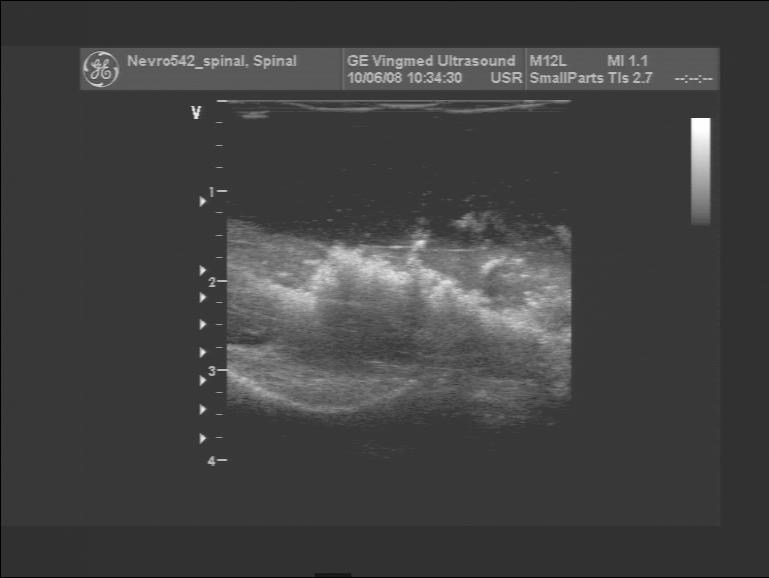
\includegraphics[width=0.49\textwidth]{graphics/60.png}
	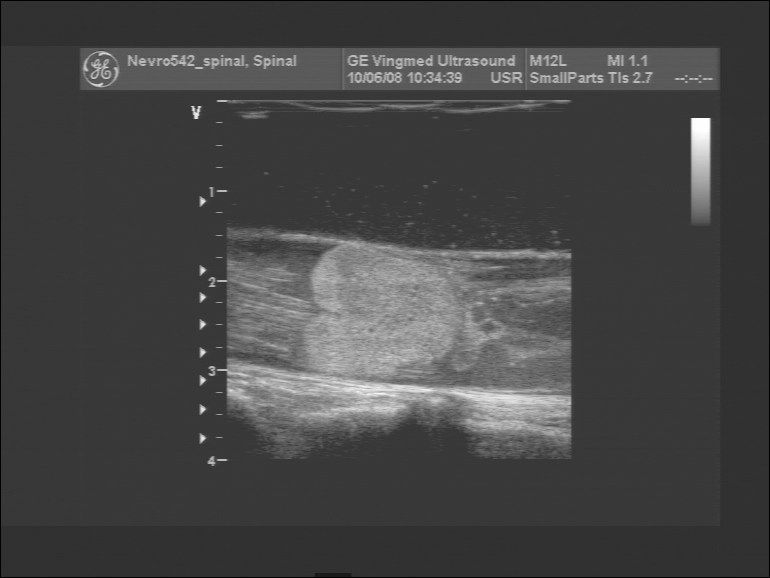
\includegraphics[width=0.49\textwidth]{graphics/280.png}
	\caption[B-scan examples from input set]{B-scan number 60 and 225 of the input set given in Table \ref{table:test_input}}
	\label{fig:example_b-scans}
	\end{figure}
	
	\begin{figure}[h]
	\centering
	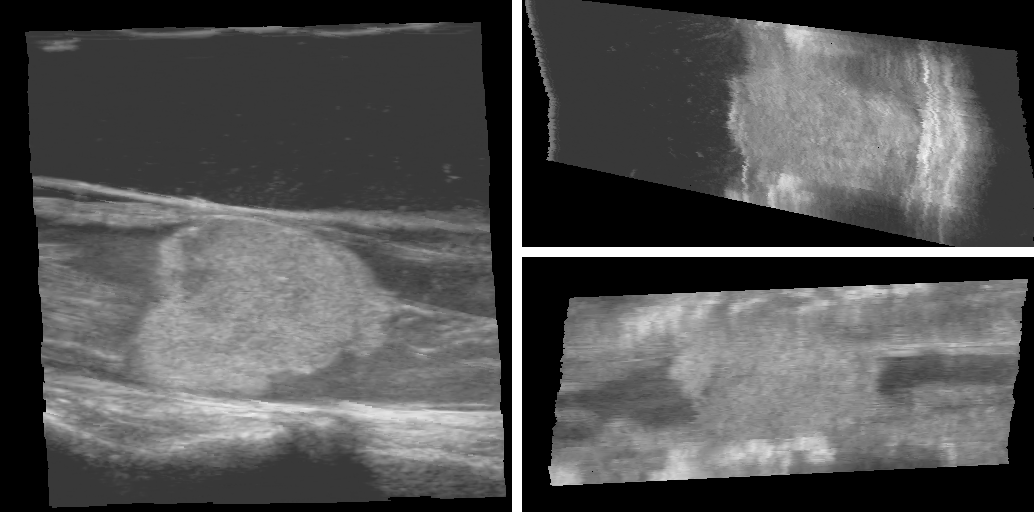
\includegraphics[width=\textwidth]{graphics/example_volume.png}
	\caption[Example volume]{Example of three orthogonal slices of a reconstructed volume (left: X-axis, top-right: Z-axis, bottom-right: Y-axis) generated by our implementation}
	\label{fig:example_volume}
	\end{figure}

% discuss what is meant by quality (close to ground truth, fact: input data less than output data, averaging blurs, tradeoff between hidden positives and false positives)
\subsection{What is Quality}

	It is difficult to define a scale for a qualitative measure such as reconstruction quality. The goal of reconstruction is to be as close to the ground truth as possible, but the reality is that given a ROI of $342 \times 356$ bytes over 434 b-scans and an output volume of $512 \times 256 \times 512$ bytes, the input is only 79 \% of the output. This means that in the case of our test data, even with a perfect reconstruction algorithm, the true volume cannot be calculated as some interpolation is required.
	
	So given that the volume will be an estimate, the discussion is what the \emph{best} estimate is, and this also depends on how the volume will be used. Ultrasound scans are analyzed by trained medical personnel, and one of the main uses of the reconstructed volume is to be examined by such people. There is an important tradeoff between avoiding false positives and hiding true positives. A false positive is an artifact of the data set that the analyzer can misinterpret as some symptom that in fact do not exist, while a hidden true positive is an actual existing artifact that is not noticeable by the analyzer. Both cases are unwanted. However, one can argue that the latter case is more important to avoid.
	
	%The various techniques for filling the missing data usually employ some sort of averaging or interpolation. Furthermore, unwanted noise in the input can be reduced by averaging redundant data. Such averaging has the advantage of reducing false positives due to noise or imperfect reconstruction schemes, but it can also hide true positives.

% discuss effect of noise in tracking data with lines.vol example
\subsection{Effect of Noise in Tracking Data}

	\begin{figure}[h]
	\centering
	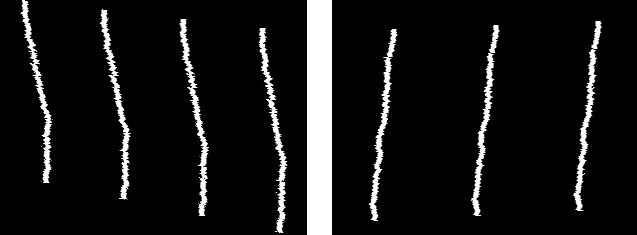
\includegraphics[width=\textwidth]{graphics/tracking_noise.png}
	\caption[Noise in the tracking data]{Noise in the tracking data seen in reconstructed volume (left: seen along Z-axis, right: seen along X-axis) generated by our implementation}
	\label{fig:tracking_noise}
	\end{figure}

	Any reconstruction method can only be as good as the input it is given. For the input data used in this thesis, the quality of the ultrasound b-scan images was more than adequate compared to the quality of the tracking data. For the test data used in this chapter, the ROI is $3.7 \times 4.0$ cm in world space, and the freehand movement covers a stretch of about 2 cm. When dealing with such small sizes, inaccuracies in the tracking can be expected. Figure \ref{fig:tracking_noise} shows the result of reconstructing images of straight lines using the tracking data. One can clearly see the oscillating disruption from the general probe trajectory. The effect is especially noticeable because of the small distances between adjacent scans.
	
	A plausible explanation could be that the freehand movement of the probe actually was jittery (e.g.\ an unsteady hand), but if one would look at the input b-scans before reconstruction, one would see that details are preserved on the same location over several neighbor images without any jitters. Thus, we conclude that the accuracy of the tracking data is poor, and this affects the results of all reconstruction methods.

% discuss reconstruction quality of the various algorithms
	% grid of screens (one axis, cropped on interesting part (same for all))
	% discussion of quality of each alg, w/ various zoomings of interesting stuff to illustrate
\subsection{Reconstruction Quality Results}
	
	Figure \ref{fig:crops} shows the results of various reconstruction methods. An interesting region of the volume is cropped from the rest to make it easier to spot key differences, and uncropped large figures can be found in Appendix \ref{chapter:large_figures}. Each crop is a slice of the same area looking in the direction of the X-axis. The compounding method used for all methods is $overwrite$.
	
	\begin{figure}[h]
	\centering
	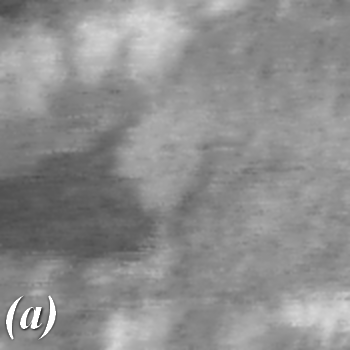
\includegraphics[width=0.48\textwidth]{graphics/crop_pnn.png}
	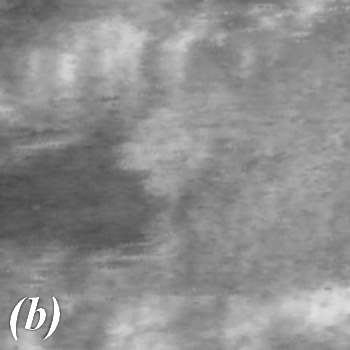
\includegraphics[width=0.48\textwidth]{graphics/crop_vnn.png}
	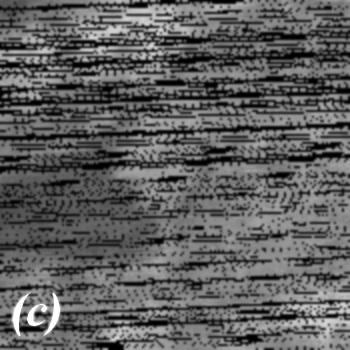
\includegraphics[width=0.48\textwidth]{graphics/crop_pnn_holes.png}
	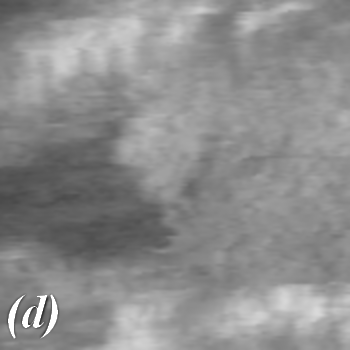
\includegraphics[width=0.48\textwidth]{graphics/crop_dwop4.png}
	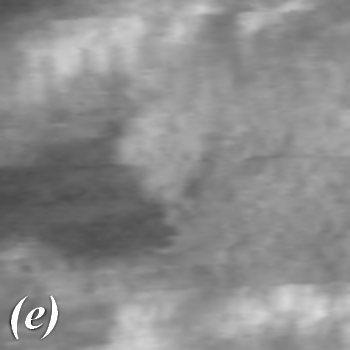
\includegraphics[width=0.48\textwidth]{graphics/crop_dwop8.png}
	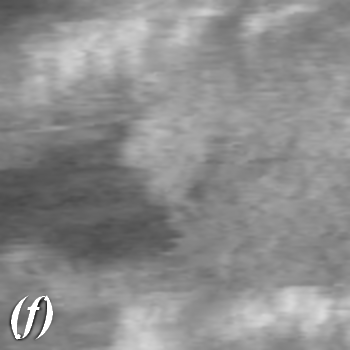
\includegraphics[width=0.48\textwidth]{graphics/crop_pt.png}
	\caption[Cropped section of reconstructed volume]{\small Cropped section of reconstructed volume generated by our implementation. \textbf{$(a)$} PNN. \textbf{$(b)$} VNN. \textbf{$(c)$} PNN w/ no hole filling. \textbf{$(d)$} incremental $DWOP_4$. \textbf{$(e)$} incremental $DWOP_8$. \textbf{$(f)$} incremental PT.}
	\label{fig:crops}
	\end{figure}
	
	\clearpage
	
	\subsubsection{PNN Quality} % also Incr PNN (PNN no hole filling)
	
		As seen in Figure \ref{fig:crops}a, the PNN is somewhat grainy, and this is expected when using only the nearest neighbor for filling instead of some method of weighting. Some of the grains are also due to the fact that there are not enough pixels to fill the entire volume. This means that along a row of pixels, at some point a voxel is skipped. E.g.\ if there are 20 pixels along a row of a b-scan, and they are reconstructed onto a voxel that has 25 voxels along a row of the same size, then 5 voxels are periodically left empty. This is clearly seen in Figure \ref{fig:crops}c where hole filling is turned off. In addition to the black lines of holes between b-scans, there are periodical holes every 4-5 voxels in a grid because the pixel spacing is $\simeq 0.1$, while the voxel spacing is $0.08$, i.e.\ $\frac{0.1}{0.08} = 1 \frac{1}{4}$. Additionally, one can also see the tendency for horizontal lines in the image, but this is mainly due to the tracking noise discussed earlier, and is present in all cases.
	
	\subsubsection{VNN Quality}
	
		One can see in Figure \ref{fig:crops}b that the VNN is sharper than the PNN. More details are preserved in the white spots at the top, and the texture of the gray area at the right is more clearly visible. This can be caused by the smoothing effect of averaging voxels when filling the PNN holes. The VNN method is still based on nearest-neighbor however, and also suffers from graining as the PNN method. This is unavoidable as two neighboring voxels often have different closest b-scans when the scans are packed together.
	
	\subsubsection{Incremental DWOP Quality} % DWOP4 and DWOP8
	
		$DWOP_4$ and $DWOP_8$, shown in Figure \ref{fig:crops}d and \ref{fig:crops}e, do not have the problem of grains that occurs with PNN and VNN. This is of course because several b-scans influence each voxel, and those b-scans are weighted differently. The drawback, however, is a slightly noticeable blurring of the volume when compared to VNN. However, one can argue that the sharper features of VNN might be largely due to the effect of the grains, thereby effectively allowing a cluster of grains to be mistaken as a feature.
		
		The difference between $DWOP_4$ and $DWOP_8$ is not substantial, but the $DWOP_8$ is slightly smoother than the $DWOP_4$. This is explained by the fact that $DWOP_8$ weights \emph{eight} neighbor b-scans instead of \emph{four}, and thus each voxel is influenced by b-scans further away than with $DWOP_4$, causing the blurring. Since the weighting is distance based, this blur is minor, but the similarity between $DWOP_4$ and $DWOP_8$ does not justify the increase in computation time associated with $DWOP_8$.
	
	\subsubsection{Incremental PT Quality}
	
		The result of the PT method is shown in Figure \ref{fig:crops}f, and as the other weighting based methods, it does not contain grains. However, in comparison to DWOP, it is clearer and sharper, with the details of the white area at the top and the texture of the gray area to the right being superior to those from other methods. With PT having only a slightly greater computation time than $DWOP_4$ it is evident from this thesis that PT is a superior method.		
		
		To illustrate another advantage of the PT method, Figure \ref{fig:sparse} and shows the results when the input is sparse. With more space between the b-scans, the approach to filling this space becomes more important. Figure \ref{fig:sparse_lines} highlights the differences even more by using straight lines instead of ultrasound b-scans (but using the real tracking data).
		
		\begin{figure}[h]
			\centering
			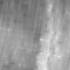
\includegraphics[height=0.2\textheight]{graphics/dwop8_sparse.png}
			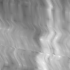
\includegraphics[height=0.2\textheight]{graphics/pt_sparse.png}
			\caption[Reconstructed sparse input]{Reconstruction of sparse input ($DWOP_8$ and PT) generated by our implementation}
			\label{fig:sparse}
		\end{figure}
		
		As demonstrated in Figure \ref{fig:sparse}, because DWOP is based on orthogonal projections, one can clearly see tendencies for straight lines at approximately an 80 degrees angle. These lines are orthogonal to the b-scan plane normals. PT uses cubic interpolation along the probe trajectory, and one can see how the features curve along the tracked path (with tracking noise).
		
		With the straight lines of Figure \ref{fig:sparse_lines}, one can also see how the PT is superior in filling in values between sparse b-scans. The reconstructed line from DWOP appears discontinuous across the adjacent planes. PT in contrast, preserves the intensity of the line along the probe trajectory.
		
		\begin{figure}[h]
			\centering
			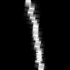
\includegraphics[height=0.2\textheight]{graphics/dwop8_sparse_lines.png}
			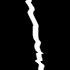
\includegraphics[height=0.2\textheight]{graphics/pt_sparse_lines.png}
			\caption[Reconstructed sparse input (straight lines)]{Reconstruction of sparse input (straight lines) ($DWOP_8$ and PT) generated by our implementation}
			\label{fig:sparse_lines}
		\end{figure}

% discuss effect of various compounding methods
	% grid with examples
\subsection{Effect of Compounding Methods}

	\begin{figure}[h]
	\centering
	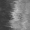
\includegraphics[width=0.24\textwidth]{graphics/overwrite.png}
	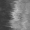
\includegraphics[width=0.24\textwidth]{graphics/avg.png}
	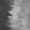
\includegraphics[width=0.24\textwidth]{graphics/max.png}
	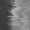
\includegraphics[width=0.24\textwidth]{graphics/ifempty.png}
	\caption[Result of compounding methods]{Result of compounding methods generated by our implementation: $overwrite$, $avg$, $max$ and $ifempty$ (PT method)}
	\label{fig:compounding methods}
	\end{figure}
	
	Figure \ref{fig:compounding methods} shows the effect of each of the four compounding methods as presented in Table \ref{table:compounding_methods}: $overwrite$, $avg$, $max$ and $ifempty$. Larger uncropped figures can be found in Appendix \ref{chapter:large_figures}. As expected, the $avg$ method slightly blurs the output compared to $overwrite$, but since the averaging occurs internally in each voxel, the details and features persist.
	
	The $max$ method is smoother and brighter than the others. This is the case since only the brightest voxel values are kept, resulting in an overall brighter output. Some details are lost, however, when comparing to the two previous methods, and this can be explained by the fact that a single bright voxel value will dominate any set of darker values for that voxel. With some noise in the tracking, a bright pixel will thus "spread out", resulting in smoother transitions.
	
	The result of $ifempty$ is somewhat different than $overwrite$ and $avg$, and one can see some features appear in this method that do not appear in the results of $overwrite$ and $avg$. The main difference between these methods is that $overwrite$ keeps the \emph{latest} value of a voxel, $ifempty$ keeps the \emph{first} value, and $avg$ averages them all. Given that $overwrite$ and $avg$ so similar, it can be speculated that the last voxel values are more "correct" than the first values. Noise in the tracking data should be just as likely to cause jitter forward as well as backward, and so it is believed to be a property of the incremental reconstruction method.